%!TEX root = Thesis.tex

\chapter{Coordination Complexes with Platinum and Palladium}
\label{ch:platinum}

Previous work with wide bite-angle ligands based on xanthene backbones has encountered difficulties when attempting coordination to Pt and Pd(II).  The reactions proceed giving either a mixture of products\cite{Malaise2006, Veen2000b} or dynamic processes \cite{Veen2000b}.  The square planar geometries preferred by these metals allows for either \emph{cis} or \emph{trans} coordination allowing for bite-angles of 90 or 180\degrees{}.  The xanthene based ligands have bite-angles of generally around 120\degrees{} and limited flexibility.  Hence often both \emph{cis} and \emph{trans} complexes form or an interconversion between the two is observed.  As such more work has been carried out with metals that are less rigid in their coordination geometries, such as Rh.  

Platinum xantphos complexes have shown particular activity in the allylation of amines.\cite{Mora2008}

Petocz2004 for information on cis and trans platinum xantphos complexes

\section{Reactions with Platinum(0) Precursors}
A number of different platinum(0) precursors have been utilised in this work.  Due to the lack of characterised platinum(0) complexes of the widely used xantphos ligands a reaction between thixantphos and \emph{tris}-norborneneplatinum was carried out.  When an equimolar ratio of the ligand and the metal precusor were combined a mixture of products were formed, together with remaining \emph{tris}-norborneneplatinum (Scheme \ref{thixantphos+Pt(nb)3}).  This led to the proposal that one of the complexes was \emph{bis}-thixantphosplatinum.  The reaction was repeated with two equivalents of ligand and this complex was formed exclusively, allowing for full characterisation.  The remaining complex was formulated as thixantphos platinum norbornene.  

\begin{scheme}[h]
\begin{center}
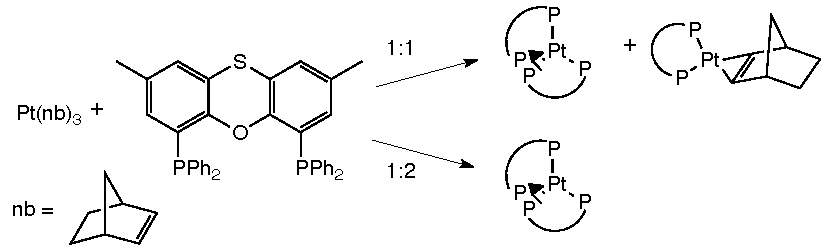
\includegraphics{../Schemes/thixantphosPtnb3.pdf}
\caption[Reaction of thixantphos with \emph{tris}-norborneneplatinum]{Reaction of thixantphos with \emph{tris}-norborneneplatinum}
\label{thixantphos+Pt(nb)3}
\end{center}
\end{scheme}

\emph{bis}-Thixantphosplatinum shows an unusual pattern in the \phosphorus{} NMR spectrum.  At room temperature a single broad signal is present.  When cooled this resolves into two triplets.  This indicates that there are two different phosphorus environments in the molecule that couple to each other, however in solution at room temperature the sufficient energy is present to allow interconversion. \fixme{add some values for coupling constants etc}.

Single yellow crystals of \fixme{bis-thixantphosplatinum} suitable for X-ray crystallography were grown by inwards diffusion of diethyl into a dichloromethane solution of \fixme{bis-thixantphosplatinum} in the air.  \fixme{some stuff about similar structures}  The complex crystallised as \ce{[Pt(thixantphos)2]}$\cdot$2.5 \ce{CH2Cl2} with 2$\nicefrac{1}{2}$ molecules of dichloromethane as solvate.  The X-ray crystal structure (Figure \ref{Crystal:bisthixantphosplatinum}) is in the monoclinic space group C2/c.  Selected bond lengths and angles are given in Table \ref{table:crystalbisthixantphosplatinum:lengths} and crystallographic data is given in Table \ref{table:crystalbisthixantphosplatinum:data}. 

The platinum shows a distorted tetrahedral environment with angles ranging from 103.73 to 119.321\degrees.  There are two different phosphorus environments present in the crystal structure, such that each ligand has each of the two environments.  One phosphine on each ligand is nearer to the adjacent ligand backbone whilst the other phosphine is nearer to the adjacent phenyl substituents.  The backbone is bent away from planarity to allow the ligand to coordinate with bite angles of 106.37 and 108.06\degrees. These angles are relatively close to the natural bite angle calculated for this ligand of 109.4\degrees and well within the calculated flexibility range of 94 - 130\degrees.  At room temperature the molecule will have sufficient energy to invert the backbone which would result in the phosphorus environments switching.  Hence in the \phosphorus{} NMR spectrum we only see the average of the two environments.  

\fixme{get ratios of the two complexes that are formed}

\begin{figure}[ht]
\begin{center}
\includegraphics[width=0.8\textwidth]{../Figures/Crystalbisthixantphosplatinum.pdf}
\caption[X-ray crystal structure of \ce{[StBu-xantphos(H)]CPh(SO2CF3)2}]{X-ray crystal structure of \ce{[StBu-xantphos(H)]CPh(SO2CF3)2}$\cdot{}$ \nicefrac{1}{2}\ce{C6D6}.  Benzene solvent of crystallisation and hydrogen atoms omitted for clarity}
\label{Crystal:bisthixantphosplatinum}
\end{center}
\end{figure}

\begin{table}[ht]
\caption[Selected bond distances (\AA) and angles (\degrees) of \ce{StBu-xantphos(H)]CPh(SO2CF3)2}$\cdot{}$ \nicefrac{1}{2}\ce{C6D6}]{Selected bond distances (\AA) and angles (\degrees) of \ce{StBu-xantphos(H)]CPh(SO2CF3)2}$\cdot{}$ \nicefrac{1}{2}\ce{C6D6}} 
\label{table:crystalbisthixantphosplatinum:lengths}
\begin{center}
\begin{tabular}{l l l l}
	\toprule
	\multicolumn{2}{l}{\bfseries{~Bond distances (\si{\angstrom})}} & \multicolumn{2}{c}{\bfseries{Bond angles (\degrees)}} \\
	\midrule		
	~P1-P2		~~&~~3.722~~	&~~P1-Pt-P2			&~~106.36(5)~~	\\	
	~P3-P4		~~&~~3.766~~	&~~P3-Pt-P4			&~~108.06(0)~~	\\
	~P1-Pt		~~&~~2.325~~	&~~P1-Pt-P3			&~~103.72(6)~~	\\
	~P2-Pt		~~&~~2.324~~	&~~P1-Pt-P4			&~~119.321~~		\\
	~P3-Pt		~~&~~2.322~~	&~~P2-Pt-P3			&~~114.239~~		\\
	~P4-Pt		~~&~~2.331~~	&~~P2-Pt-P4			&~~105.506~~		\\
	~O1-Pt		~~&~~3.565~~	&~~Ring 1-Ring 2		&~~XXXX~~		\\
	~O2-Pt		~~&~~3.497~~	&~~Ring 3-Ring 4		&~~XXXX~~		\\
%	~P1-O2		~~&~~XXXX~~	&~~					&~~XXXX~~	\\
%	~P2-O2		~~&~~XXXX~~	&~~					&~~XXXX~~	\\
%	~P3-O1		~~&~~XXXX~~	&~~					&~~XXXX~~	\\
%	~P4-O1		~~&~~XXXX~~	&~~					&~~XXXX~~	\\
	\bottomrule{}
\label{table:crystalprotonated:lengths}
\end{tabular}
\end{center}
\end{table}

\begin{table}[htp]
\caption[Crystallographic data of \ce{StBu-xantphos(H)]CPh(SO2CF3)2}$\cdot{}$ \nicefrac{1}{2}\ce{C6D6}]{Crystallographic data of \ce{StBu-xantphos(H)]CPh(SO2CF3)2}$\cdot{}$ \nicefrac{1}{2}\ce{C6D6}} 
\label{table:crystalbisthixantphosplatinum:data}
\begin{center}
\begin{tabular}{l l}
	\toprule
	~~\bfseries{Empirical formula}~~&~~\fixme{XXXXX}\\
	\midrule	
	~~Formula weight~~		&~~XXX~~	\\
	~~Crystal system~~		&~~XXX~~	\\
	~~Space group~~		&~~XXX~~	\\
	~~a$/$\si{\angstrom}~~	&~~XXX~~	\\
	~~b$/$\si{\angstrom}~~	&~~XXX~~	\\
	~~c$/$\si{\angstrom}~~	&~~XXX~~	\\
	~~$\alpha/$\degrees~~	&~~XXX~~	\\
	~~$\beta/$\degrees~~	&~~XXX~~	\\
	~~$\gamma/$\degrees~~	&~~XXX~~	\\
	~~V$/$\si{\angstrom\cubed}&~~XXX~~	\\
	~~Z					&~~XXX~~	\\
	~~Cell determination reflections &~~XXX~~	\\
	~~Cell determination range, $\theta{}$\textsubscript{min} $\longrightarrow \theta{}$\textsubscript{max}/\degrees &~~XXX~~	\\
	~~Temperature $/$\si{\kelvin}	&~~XXX~~	\\
	~~Radiation type			&~~XXX~~	\\
	~~Radiation ($\lambda$) $/$\si{\angstrom}	&~~XXX~~	\\
	~~Crystal size $/$\si{\milli\metre}			&~~XXX~~	\\
	~~D\textsubscript{\emph{calc}} $/$ \si{\gram\per\metre\cubed}	&~~XXX~~	\\
	~~F(000)				&~~XXX~~	\\
	~~$\mu /$	\si{\per\milli\metre}		&~~XXX~~	\\
	~~Experimental absorption correction type	&~~XXX~~	\\
	~~T\textsubscript{max}, T\textsubscript{min}	&~~XXX~~	\\
	~~Reflections collected					&~~XXX~~	\\
	~~Index range \emph{h}		&~~XXX~~	\\
	~~Index range \emph{k}		&~~XXX~~	\\
	~~Index range \emph{l}		&~~XXX~~	\\
	~~$\theta$ range $/$\degrees	&~~XXX~~	\\
	~~Independent reflections		&~~XXX~~	\\
	~~Reflections $[\emph{I} > 2\sigma(\emph{I})]$	&~~XXX~~	\\
	~~Restraints $/$ parameters	&~~XXX~~	\\
	~~GOF					&~~XXX~~	\\
	~~R\textsubscript{1} $[\emph{I} > 2\sigma(\emph{I})]$	&~~XXX~~	\\
	~~wR2 $[\emph{I} > 2\sigma(\emph{I})]$	&~~XXX~~	\\
	~~R\textsubscript{1} [all data]	&~~XXX~~	\\
	~~wR2 [all data]			&~~XXX~~	\\
	~~Residual density $/$e \si{\per\angstrom\cubed}	&~~XXX~~	\\
	\bottomrule{}
\end{tabular}
\end{center}
\end{table}

\fixme{check if tris should be italicised}
\fixme{replaced this horrible structure with a better one}

When the reaction between \emph{tris}-norbornene platinum was carried out with the tertiary butyl substituted thixantphos a different result was observed.  Similarly to the reaction with the phenyl derivative an initial mixture of products was obtained.  In this case both are 1:1 complexes tBu-thixantphos:platinum.  Like the phenyl derivative one of the products is platinum thixantphos norbornene.  The other product is the two-coordinate 14-electron complex platinum thixantphos (Scheme \ref{scheme:StBuPtnb}).  \fixme{give references to these things}  

%The platinum norbornene complex exists only in the presence of excess norbornene and can readily be converted to the 14-electron complex by removing the norbornene \emph{in vacuo}.  

\begin{scheme}[ht]
\begin{center}
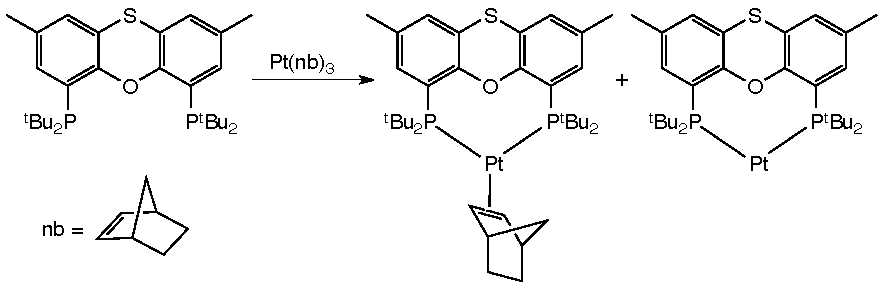
\includegraphics{../Schemes/StBuPtnb.pdf}
\caption[Reaction between tBu-thixantphos and \emph{tris}-norborneneplatinum]{Reaction between tBu-thixantphos and \emph{tris}-norborneneplatinum.}
\label{scheme:StBuPtnb}
\end{center}
\end{scheme}

%\fixme{Why is there a random black spot between my scheme and my caption?}

The initially formed norbornene complex \fixme{reference} exhibits a broad resonance at 55.63 ppm in the \phosphorus{} NMR spectrum with platinum satellites of 3612 Hz.  This value is typical for tridentate platinum alkene complexes. As this complex exists in an equilibrium with the 14-electron complex and is only present with excess norbornene the norbornene NMR signals are broad and some are obscured by other peaks.  The alkene protons appear at 2.37 ppm as a broad singlet with no discernable phosphorus coupling but platinum coupling of 67.8 Hz, and a similarly broad singlet in the \carbon{} NMR spectrum at 51.91 ppm with \JPtC{} = 343.9 Hz.  Half of the expected number of norbornene NMR signals are observed indicating a symmetrical complex.  Removing the excess norbornene \fixme{in vacuo} from the reaction mixture results in the exclusive formation of the two-coordinate, 14-electron platinum tBu-thixantphos complex.\fixme{ref}

The 14-electron complex \fixme{give a reference thing here} exhibits a single peak in the \phosphorus{} NMR spectrum at 78.5 ppm with a very large platinum coupling constant of 4809.5 Hz.  This value is indicative of a two-coordinate platinum(0) complex.  Several previous examples of 14-electron platinum(0) complexes have been reported.\cite{Goel1981c, Otsuka1976}  They typically form with large sterically bulky phosphines such as P\textsuperscript{t}\ce{Bu3} or P\textsuperscript{t}\ce{Bu2Ph}.  The reported complex \fixme{give a reference} has a virtual triplet for the tertiary butyl protons which is indicative of \emph{trans} coordination \cite{Harris1964}.  For a diphosphine this structure is particularly unusual as the bite-angle needs to be sufficiently large and the phosphines sufficiently bulky to prevent the coordination of solvent or other small molecules.  

Ligand \fixme{ref} tBu-Thixantphos was reacted with platinum \emph{tris}-ethene In order to investigate the role of sterics on the position of the equilibrium between the norbornene complex and the 14-electron complex.  The ligand was added to freshly synthesised \emph{tris}-ethene platinum and reacted under an ethene atmosphere.  A single product was observed in the \phosphorus{} NMR spectrum at 55.7 ppm (\JPtP{} = 3899.1 Hz) which was identified as a tBu-thixantphos platinum ethene complex (Scheme \ref{scheme:StBuPtethene}).  A single signal for the ethene was observed in the \proton{} and \carbon{} NMR spectra at 2.50 ppm (\JPtH{} = 59.5 Hz) and 34.2 ppm (\JPtC{} = 223.2 Hz).  This indicates that either the ethene is freely rotating in solution or the backbone of the ligand is inverting resulting in averaged identical averaged proton environments.  

\begin{scheme}[ht]
\begin{center}
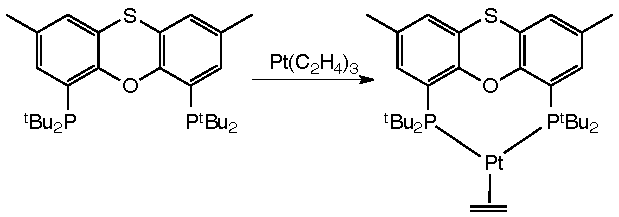
\includegraphics{../Schemes/StBuPtethene.pdf}
\caption[Reaction between tBu-thixantphos and \emph{tris}-ethene platinum]{Reaction between tBu-thixantphos and \emph{tris}-ethene platinum.}
\label{scheme:StBuPtethene}
\end{center}
\end{scheme}

A reaction between \emph{bis}-1,5-cyclooctadiene platinum and tBu-thixantphos resulted in exclusively the 14-electron complex.  However, upon completion of the reaction peaks were observed in the \proton{} and \carbon{} NMR spectra corresponding to 1,3- and 1,4-cyclooctadiene as well as 1,5-cyclooctadiene, this was further confirmed by gas chromatography mass spectrometry analysis of the sample.\fixme{get relative ratios?}  An intermediate was observed with a high field triplet in the \proton{} NMR at -18.2 ppm (\JPH{} = 13.7, \JPtH = 1100).  This indicates that the cyclooctadiene was likely undergoing a C-H activation reaction followed by isomerisation of the double bonds and then reductive elimination to give the different isomers.  

The three reactions with the alkenes show markedly different results.  With norbornene an equilibrium forms between the norbornene complex and the 14-electron complex, with \emph{bis}-COD platinum only the 14-electron complex forms and with \emph{tris}-ethene platinum only the ethene complex results.  This is contrary to what is expected given that COD is the strongest binding of the three alkenes due to the chelate effect and the NMR data for the ethene and norbornene complexes indicates that the ethene is less strongly bound to the platinum than the norbornene (\JPtC{} = 223.2 and 343.9 Hz respectively).  The presence of a large excess of ethene by working under an ethene atmosphere may be sufficient to push the equilibrium towards the ethene complex, however the reaction in both cases would produce two equivalents of excess alkene so this is unlikely to make a significant difference.  

The reason for this distinct difference between the three alkenes is likely to be predominantly sterics.  The COD is the largest of the three followed by norbornene then ethene \fixme{get cone angles or a reference or something}.  The thixantphos ligand has a calculated natural bite-angle of 131\degrees and has large tertiary butyl groups resulting in a large cone angle\fixme{probably best to get some data on this}.  As such the molecule is put under strain by the addition of larger alkenes which offset the additional stability that the alkenes afford by contributing electron density to the metal centre.  As COD is the largest of the three the final complex shows none of the alkene complex whilst the ethene as the smallest is exclusively the ethene complex.  However, norbornene being of an intermediate size forms an equilibrium with both the norbornene complex and the 14-electron complex coexisting.  

 %so there is more strain present in the molecule when the norbornene is bound compared to ethene which counteracts the added stability from having a 16-electron metal centre.  This strain results in a higher energy complex with little barrier to norbornene loss and little energy different between the norbornene complex and the 14-electron complex, thus resulting in an equilibrium.  In the ethene there is very little strain induced from the ethene and the additional electron density on the platinum results in the ethene complex being much lower in energy and thus no equilibrium is present between the ethene and the 14-electron complex.  

The tBu-thixantphos platinum alkene complexes and the 14-electron tBu-thixantphos platinum all react rapidly and irreversibly with oxygen to form the dioxygen complex \fixme{reference}.  The slow diffusion of oxygen into a benzene solution of the tBu-thixantphos platinum ethene complex resulted in crystals of the dioxygen complex suitable for X-ray diffraction whilst crystallisation of a solution of the 14-electron complex under argon resulted in crystals containing a mixture of the 14-electron and the dioxygen complex.  This is either a result of co-crystallisation or due to molecules at the surface of the crystal reacting with oxygen during mounting and data collection.  The dioxygen complex crystallised in the Pbca space group as [Pt(tBu-thixantphos)\ce{O2}] $\cdot{}$ \ce{2C6D6} (Figure \ref{crystal:dioxygen}).  Selected bond lengths and angles for the pure dioxygen crystals and the dioxygen and 14-electron crystals are summarised in Tables \ref{table:crystaldioxygen:lengths} and \ref{table:crystal14electron:lengths} respectively and crystallographic data is given in Tables \ref{table:crystaldioxygen:data} and \ref{table:crystal14electron:data}.

%Crystals suitable for X-ray crystallography were obtained from a benzene solution of the 14-electron complex.  The crystals were found to contain a mixture of the 14-electron and the dioxygen complex, either co-crystallised or due to the surface of the crystal reacting with oxygen during mounting and data collection.  The data quality was poor preventing anisotropic refinement.  

\begin{figure}[ht]
\begin{center}
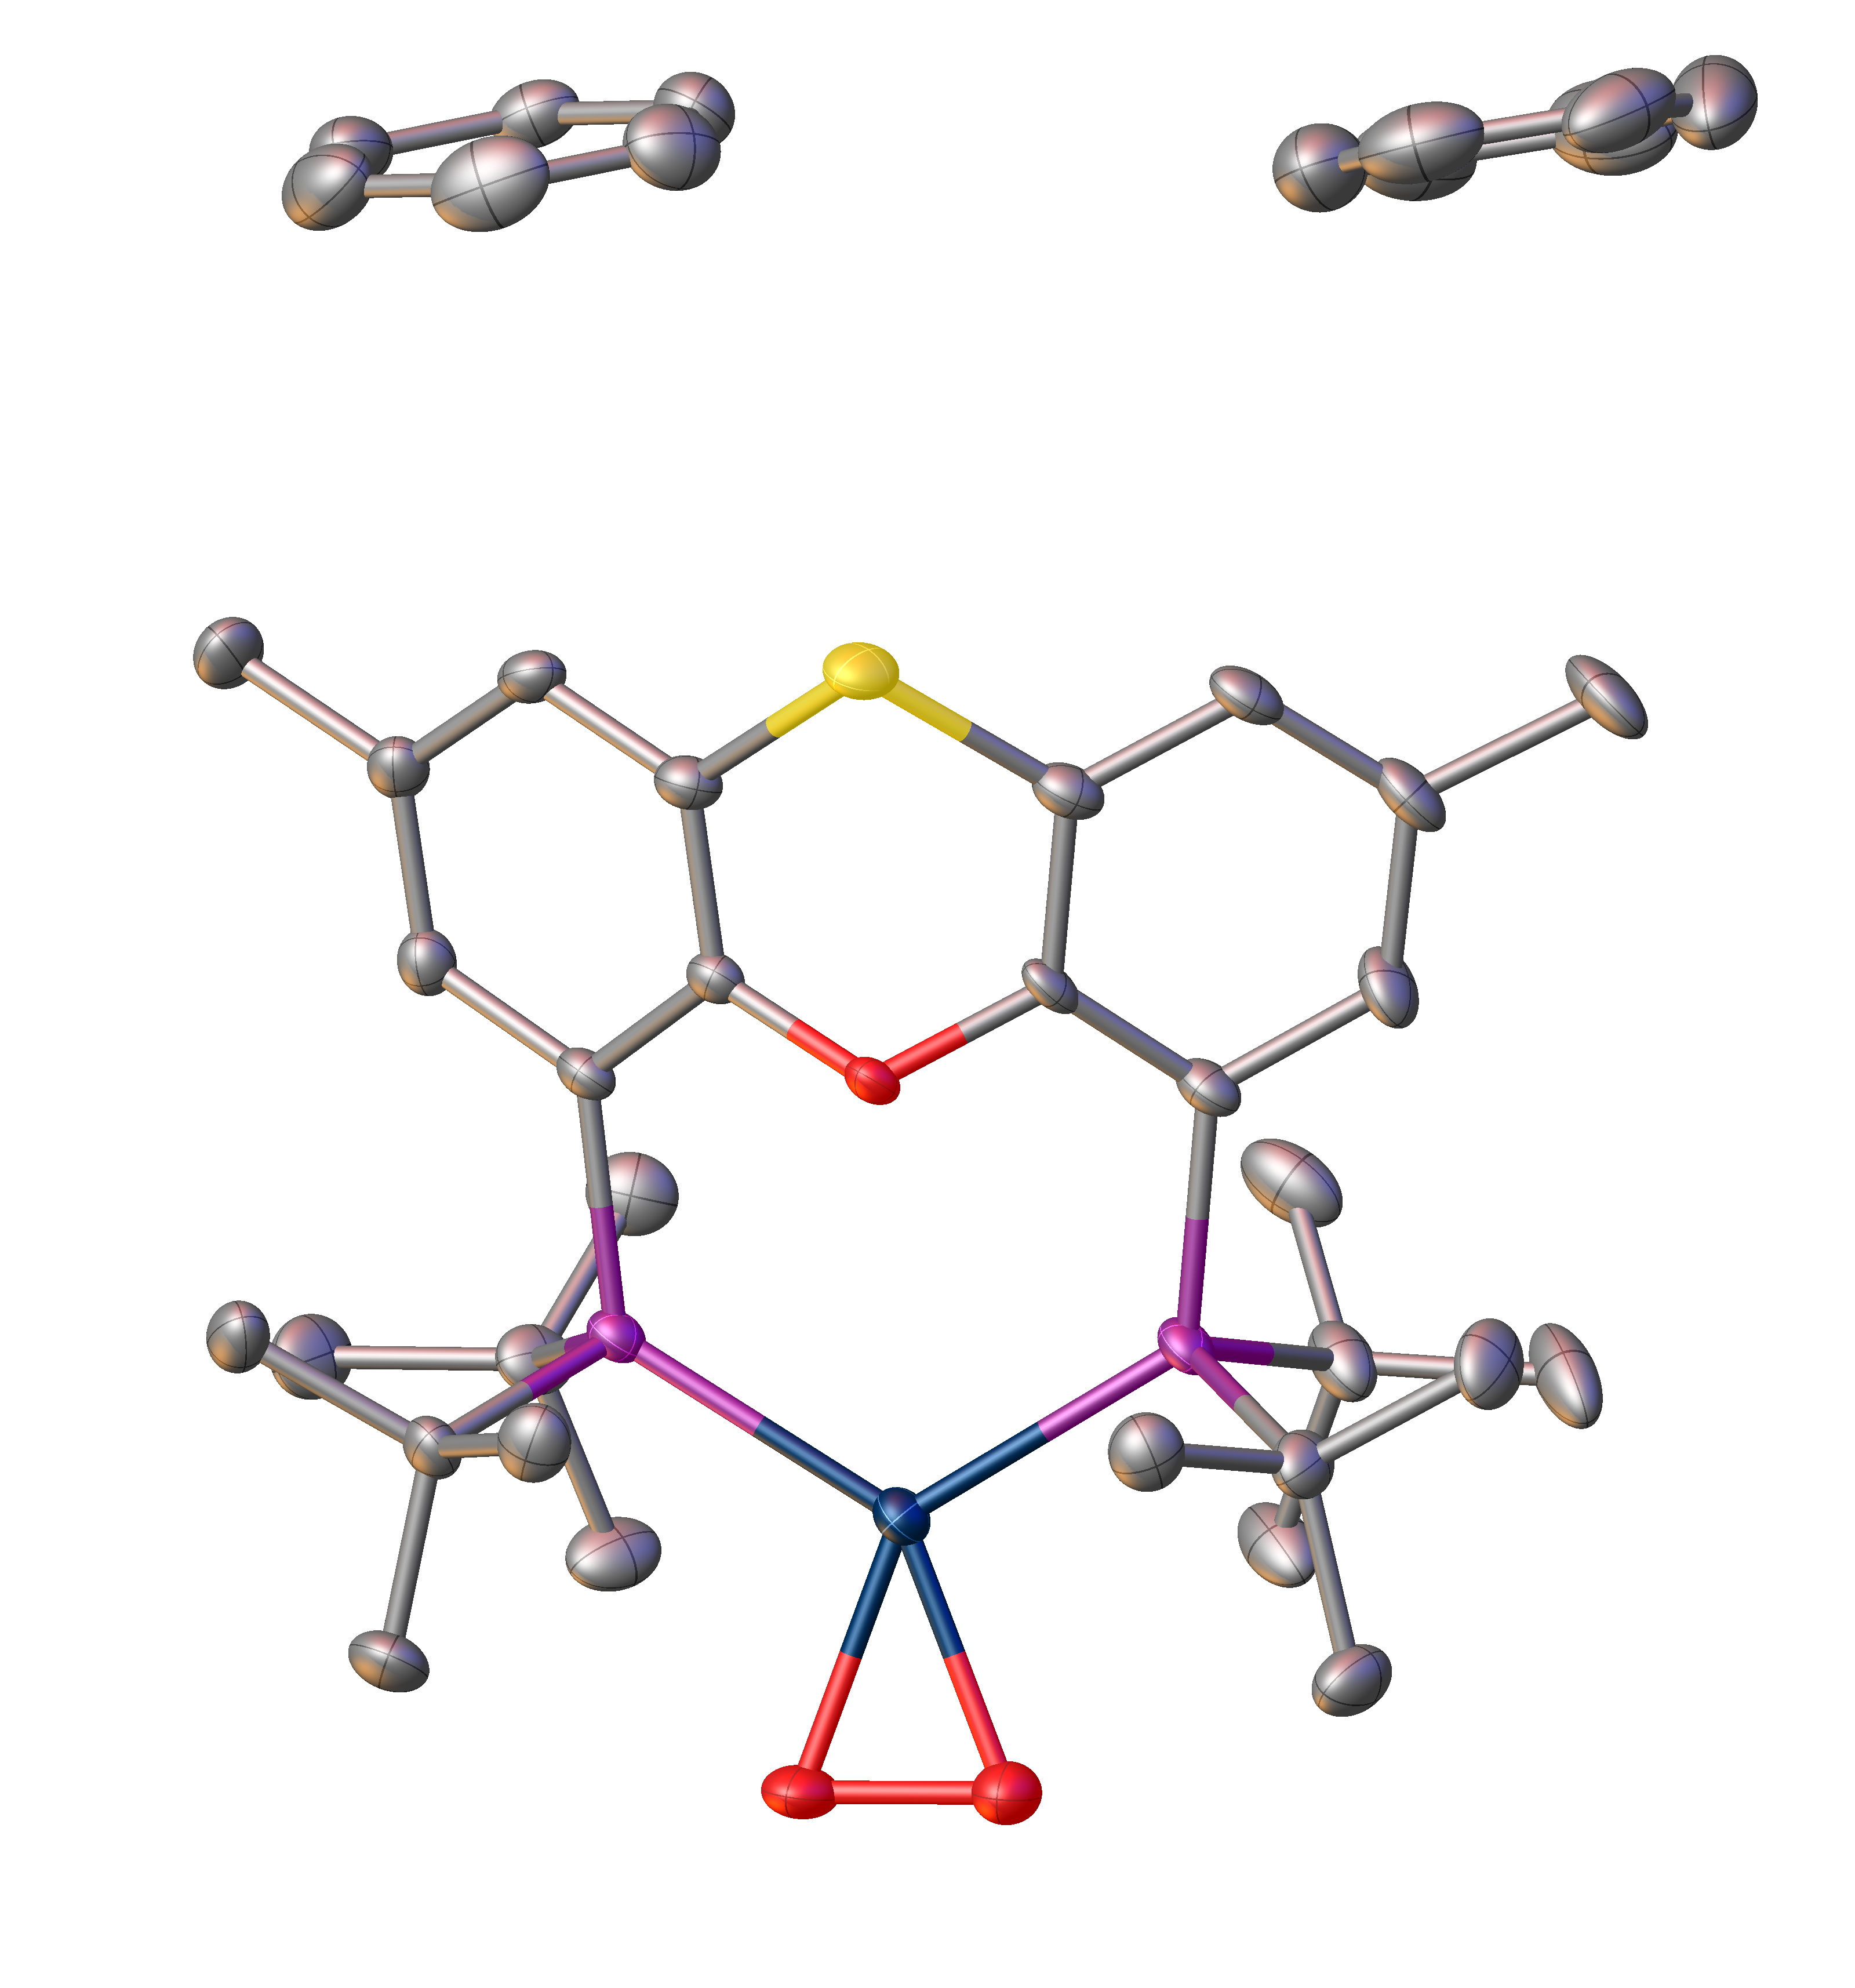
\includegraphics[width=0.8\textwidth]{../Figures/Crystaldioxygen.png}
\caption[X-ray crystal structure of [Pt(tBu-thixantphos)\ce{O2}{]} $\cdot{}$ \ce{2C6H6}]{[Pt(tBu-thixantphos)\ce{O2}] $\cdot{}$ \ce{2C6H6}.  Hydrogen atoms omitted for clarity}
\label{crystal:dioxygen}
\end{center}
\end{figure}

%dioxygen
\begin{table}[ht]
\caption[Selected bond distances (\AA) and angles (\degrees) of [Pt(tBu-thixantphos)\ce{O2}{]} $\cdot{}$ \ce{2C6H6}]{Selected bond distances (\AA) and angles (\degrees) of [Pt(tBu-thixantphos)\ce{O2}{]} $\cdot{}$ \ce{2C6H6}} 
\label{table:crystaldioxygen:lengths}
\begin{center}
\begin{tabular}{l l l l}
	\toprule
	\multicolumn{2}{l}{\bfseries{~Bond distances (\si{\angstrom})}} & \multicolumn{2}{c}{\bfseries{Bond angles (\degrees)}} \\
	\midrule		
	~P1-Pt		~~&~~1.838~~	&~~P1-Pt-P2			&~~117.25(4)~~	\\	
	~P2-Pt		~~&~~1.850~~	&~~P1-Pt-O1			&~~100.11(8)~~	\\
	~O1-Pt		~~&~~2.022~~	&~~P2-Pt-O2			&~~101.25(1)~~	\\
	~O2-Pt		~~&~~2.023~~	&~~Ring 1 - Ring 2		&~~XXXXX~~		\\
	~O3-Pt		~~&~~3.382~~	&~~					&~~		~~		\\
	~O1-O2		~~&~~1.429~~	&~~					&~~		~~		\\
	~O1-H1		~~&~~2.100~~	&~~					&~~		~~		\\
	~O2-H2		~~&~~2.160~~	&~~					&~~		~~		\\
	\bottomrule{}
\end{tabular}
\end{center}
\end{table}

%14-electron
\begin{table}[ht]
\caption[Selected bond distances (\AA) and angles (\degrees) of [Pt(tBu-thixantphos)\ce{O2}{]} and [Pt(tBu-thixantphos){]}]{Selected bond distances (\AA) and angles (\degrees) of [Pt(tBu-thixantphos)\ce{O2}{]} and [Pt(tBu-thixantphos)]} 
\label{table:crystal14electron:lengths}
\begin{center}
\begin{tabular}{l l l l}
	\toprule
	\multicolumn{2}{l}{\bfseries{~Bond distances (\si{\angstrom})}} & \multicolumn{2}{c}{\bfseries{Bond angles (\degrees)}} \\
	\midrule		
	~P1-Pt		~~&~~1.838~~	&~~P1-Pt-P2			&~~117.25(4)~~	\\	
	~P2-Pt		~~&~~1.850~~	&~~P1-Pt-O1			&~~100.11(8)~~	\\
	~O1-Pt		~~&~~2.022~~	&~~P2-Pt-O2			&~~101.25(1)~~	\\
	~O2-Pt		~~&~~2.023~~	&~~Ring 1 - Ring 2		&~~XXXXX~~		\\
	~O3-Pt		~~&~~3.382~~	&~~					&~~		~~		\\
	~O1-O2		~~&~~1.429~~	&~~					&~~		~~		\\
	~O1-H1		~~&~~2.100~~	&~~					&~~		~~		\\
	~O2-H2		~~&~~2.160~~	&~~					&~~		~~		\\
	\bottomrule{}
\end{tabular}
\end{center}
\end{table}

%dioxygen
\begin{table}[htp]
\caption[Crystallographic data of [Pt(tBu-thixantphos)\ce{O2}{]} $\cdot{}$ \ce{2C6H6}]{Crystallographic data of [Pt(tBu-thixantphos)\ce{O2}{]} $\cdot{}$ \ce{2C6H6}} 
\label{table:crystaldioxygen:data}
\begin{center}
\begin{tabular}{l l}
	\toprule
	~~\bfseries{Empirical formula}~~&~~\ce{C30H46O3P2PtS} $\cdot{}$ 2\ce{C6H6}\\
	\midrule	
	~~Formula weight~~		&~~899.97~~	\\
	~~Crystal system~~		&~~orthorhombic~~	\\
	~~Space group~~		&~~Pbca~~	\\
	~~a$/$\si{\angstrom}~~	&~~17.7892(3)~~	\\
	~~b$/$\si{\angstrom}~~	&~~15.8129(3)~~	\\
	~~c$/$\si{\angstrom}~~	&~~28.4025(5)~~	\\
	~~$\alpha/$\degrees~~	&~~90.00~~	\\
	~~$\beta/$\degrees~~	&~~90.00~~	\\
	~~$\gamma/$\degrees~~	&~~90.00~~	\\
	~~V$/$\si{\angstrom\cubed}&~~7989.6(2)~~	\\
	~~Z					&~~8~~	\\
	~~Cell determination reflections &~~XXX~~	\\
	~~Cell determination range, $\theta{}$\textsubscript{min} $\longrightarrow \theta{}$\textsubscript{max}/\degrees &~~XXX~~	\\
	~~Temperature $/$\si{\kelvin}	&~~XXX~~	\\
	~~Radiation type			&~~XXX~~	\\
	~~Radiation ($\lambda$) $/$\si{\angstrom}	&~~XXX~~	\\
	~~Crystal size $/$\si{\milli\metre}			&~~XXX~~	\\
	~~D\textsubscript{\emph{calc}} $/$ \si{\gram\per\metre\cubed}	&~~XXX~~	\\
	~~F(000)				&~~XXX~~	\\
	~~$\mu /$	\si{\per\milli\metre}		&~~XXX~~	\\
	~~Experimental absorption correction type	&~~XXX~~	\\
	~~T\textsubscript{max}, T\textsubscript{min}	&~~XXX~~	\\
	~~Reflections collected					&~~XXX~~	\\
	~~Index range \emph{h}		&~~XXX~~	\\
	~~Index range \emph{k}		&~~XXX~~	\\
	~~Index range \emph{l}		&~~XXX~~	\\
	~~$\theta$ range $/$\degrees	&~~XXX~~	\\
	~~Independent reflections		&~~XXX~~	\\
	~~Reflections $[\emph{I} > 2\sigma(\emph{I})]$	&~~XXX~~	\\
	~~Restraints $/$ parameters	&~~XXX~~	\\
	~~GOF					&~~XXX~~	\\
	~~R\textsubscript{1} $[\emph{I} > 2\sigma(\emph{I})]$	&~~XXX~~	\\
	~~wR2 $[\emph{I} > 2\sigma(\emph{I})]$	&~~XXX~~	\\
	~~R\textsubscript{1} [all data]	&~~XXX~~	\\
	~~wR2 [all data]			&~~XXX~~	\\
	~~Residual density $/$e \si{\per\angstrom\cubed}	&~~XXX~~	\\
	\bottomrule{}
\end{tabular}
\end{center}
\end{table}

%\begin{figure}[ht]
%\begin{center}
%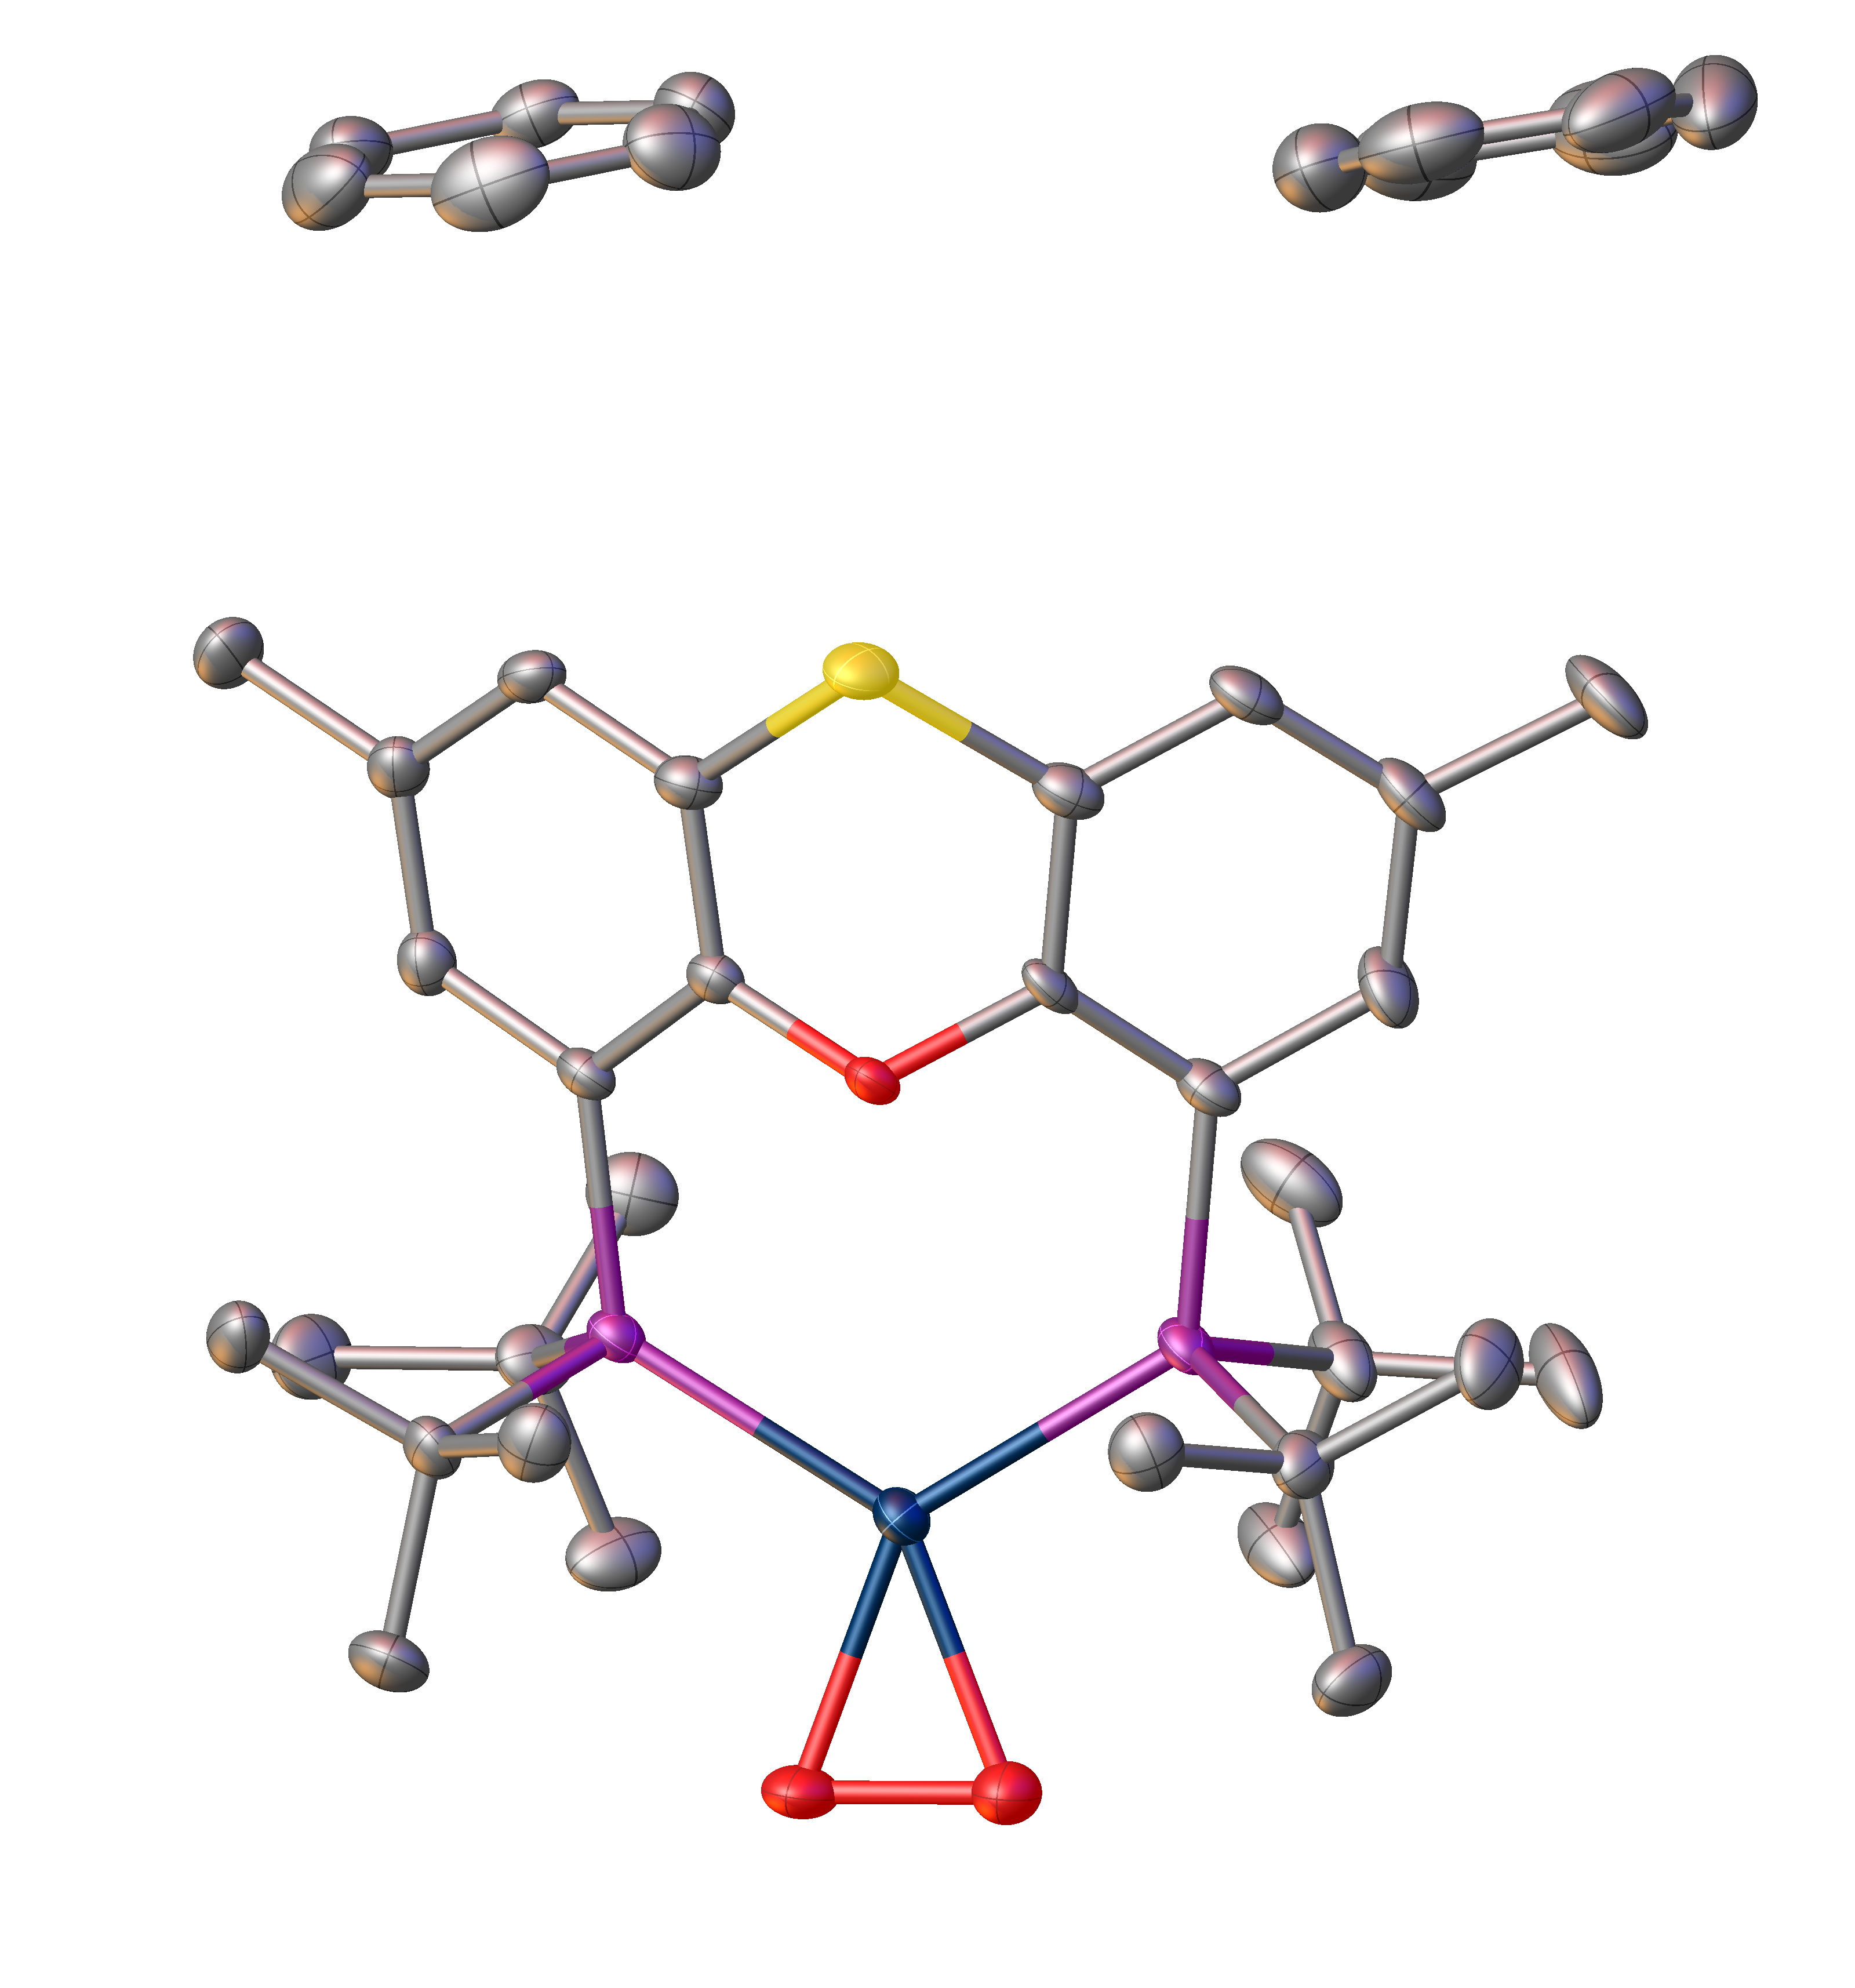
\includegraphics[width=0.8\textwidth]{../Figures/Crystaldioxygen.png}
%\caption[X-ray crystal structure of [Pt(tBu-thixantphos)\ce{O2}{]} $\cdot{}$ \ce{2C6H6}]{[Pt(tBu-thixantphos)\ce{O2}] $\cdot{}$ \ce{2C6H6}.  Hydrogen atoms omitted for clarity}
%\label{crystal:dioxygen}
%\end{center}
%\end{figure}

%14-electron
\begin{table}[htp]
\caption[Crystallographic data of [Pt(tBu-thixantphos)\ce{O2}{]} and [Pt(tBu-thixantphos){]}]{Crystallographic data of [Pt(tBu-thixantphos)\ce{O2}{]} and [Pt(tBu-thixantphos){]}} 
\label{table:crystal14electron:data}
\begin{center}
\begin{tabular}{l l}
	\toprule
	~~\bfseries{Empirical formula}~~&~~\ce{C30H46O3P2PtS} $\cdot{}$ 2\ce{C6H6}\\
	\midrule	
	~~Formula weight~~		&~~XXX~~	\\
	~~Crystal system~~		&~~XXX~~	\\
	~~Space group~~		&~~XXX~~	\\
	~~a$/$\si{\angstrom}~~	&~~XXX~~	\\
	~~b$/$\si{\angstrom}~~	&~~XXX~~	\\
	~~c$/$\si{\angstrom}~~	&~~XXX~~	\\
	~~$\alpha/$\degrees~~	&~~XXX~~	\\
	~~$\beta/$\degrees~~	&~~XXX~~	\\
	~~$\gamma/$\degrees~~	&~~XXX~~	\\
	~~V$/$\si{\angstrom\cubed}&~~XXX~~	\\
	~~Z					&~~XXX~~	\\
	~~Cell determination reflections &~~XXX~~	\\
	~~Cell determination range, $\theta{}$\textsubscript{min} $\longrightarrow \theta{}$\textsubscript{max}/\degrees &~~XXX~~	\\
	~~Temperature $/$\si{\kelvin}	&~~XXX~~	\\
	~~Radiation type			&~~XXX~~	\\
	~~Radiation ($\lambda$) $/$\si{\angstrom}	&~~XXX~~	\\
	~~Crystal size $/$\si{\milli\metre}			&~~XXX~~	\\
	~~D\textsubscript{\emph{calc}} $/$ \si{\gram\per\metre\cubed}	&~~XXX~~	\\
	~~F(000)				&~~XXX~~	\\
	~~$\mu /$	\si{\per\milli\metre}		&~~XXX~~	\\
	~~Experimental absorption correction type	&~~XXX~~	\\
	~~T\textsubscript{max}, T\textsubscript{min}	&~~XXX~~	\\
	~~Reflections collected					&~~XXX~~	\\
	~~Index range \emph{h}		&~~XXX~~	\\
	~~Index range \emph{k}		&~~XXX~~	\\
	~~Index range \emph{l}		&~~XXX~~	\\
	~~$\theta$ range $/$\degrees	&~~XXX~~	\\
	~~Independent reflections		&~~XXX~~	\\
	~~Reflections $[\emph{I} > 2\sigma(\emph{I})]$	&~~XXX~~	\\
	~~Restraints $/$ parameters	&~~XXX~~	\\
	~~GOF					&~~XXX~~	\\
	~~R\textsubscript{1} $[\emph{I} > 2\sigma(\emph{I})]$	&~~XXX~~	\\
	~~wR2 $[\emph{I} > 2\sigma(\emph{I})]$	&~~XXX~~	\\
	~~R\textsubscript{1} [all data]	&~~XXX~~	\\
	~~wR2 [all data]			&~~XXX~~	\\
	~~Residual density $/$e \si{\per\angstrom\cubed}	&~~XXX~~	\\
	\bottomrule{}
\end{tabular}
\end{center}
\end{table}

The bite-angle of 117.25(4)\degrees{} is much smaller than the calculated bite angle \fixme{insert a reference here} due to the backbone bending and the \emph{cis} coordination in order to accommodate the dioxygen coordinating in an $\eta$\sub{2} fashion.  The oxygen-oxygen bond length is typical for platinum dioxygen complexes \fixme{refer to the crystallographic database and maybe give examples} and shows a slight lengthening upon coordination from 1.21 \si{\angstrom} in free \ce{O2} to 1.429 \si{angstrom} in the complex.  The oxygen atoms have close interactions with some of the tertiary butyl protons with the closest being 2.100 and 2.160 \si{\angstrom}.  This is within the sum of the van der waals radii (\fixme{1.20 or 1.09 \si{\angstrom}} for hydrogen and 1.52 \si{\angstrom} for oxygen).   

Comparing the two crystals structures for the dioxygen and the \fixme{co-crystallised} 14-electron and dioxygen complex we can see that the dioxygen complex is very similar in both cases.  \fixme{are they in the same space group?}.   For the dioxygen complex the platinum is planar with four substituents coplanar.  In the 14-electron complex we observe a bent configuration of the platinum.  Two-coordinate platinum complexes typically form linear configurations \fixme{check CCD} so the bent configuration is likely a result of the backbone restricting the bite-angle.  

\fixme{compare (overlap perhaps?) the dioxygen complexes obtained from each crystal structure}

The differences between the 14-electron and the dioxygen complexes are of particular interest.  The ligands share the same sites in the disordered structure indicating that little ligand rearrangement is necessary for the dioxygen to coordinate.  The 14-electron complex has a much larger bite-angle \fixme{value?} with the platinum sitting much closer to the ether bridge.  This nicely shows how a metal centre and the presence of other ligands can influence the bite-angle of a diphosphine, these effects are not accounted for in the widely used, theoretically obtained, natural bite-angle as defined by Casey and Whiteker\cite{Casey1990} and it is notable here that we have two complexes with very similar ligand positions have bite-angles of \fixme{this and this} while the natural bite angle was calculated as \fixme{this}.

\fixme{check the above paragraphs once the crystal structure is back from Martyn}

\fixme{Need to check consistency of bite-angle vs. bite angle}

In order to investigate the activation of the oxygen that occurred upon coordination a number of reactions were carried with the dioxygen complex and other small molecules.  It is unreactive towards ethene and ethyne.  The reaction with 1,3,5-triaza-7-phosphaadamantane (PTA) yielded uncoordinated tBu-thixantphos and \ce{[Pt(PTA)4]} with consistent spectroscopic data to previous reports.\fixme{citation} 

A number of palladium dioxygen complexes have been reported to be reduced to palladium (0) 14-electron complexes using hydrogen, either as the pure gas or as a mixture with carbon monoxide such as in formylations and alkoxy carbonylations.\cite{Sergeev2010}  However, metal dioxygen complexes have been reported as reacting rapidly with carbon monoxide yielding a metal carbonate.\cite{Goel1983b}  This indicates that in general palladium dioxygen complexes preferentially react with hydrogen rather than carbon monoxide.  As such, we decided to investigate the reactivity of the platinum dioxygen complexes with both carbon monoxide and with hydrogen.  \fixme{I should actually react it with hydrogen at some point...}
  
The dioxygen complex \fixme{reference} reacts with carbon monoxide and forms a series of intermediates before a stable final product is observed (Scheme \ref{scheme:StBuPtO2andCO}).  The reaction was carried out with enriched \textsuperscript{13}CO and a number of intermediates were able to be identified.  The first product is the expected carbonate complex \fixme{reference?} \ce{[Pt(tBu-thixantphos)CO3]} with the carbonate appearing in the \carbon{} NMR spectrum at 167.85 ppm (t, 3.9 Hz, \JPtC{} = 64.4 Hz).  This is associated with a single environment in the \phosphorus{} NMR spectrum at 15.6 ppm with \JPtP{} = 4055.4 Hz.

\begin{scheme}[ht]
\begin{center}
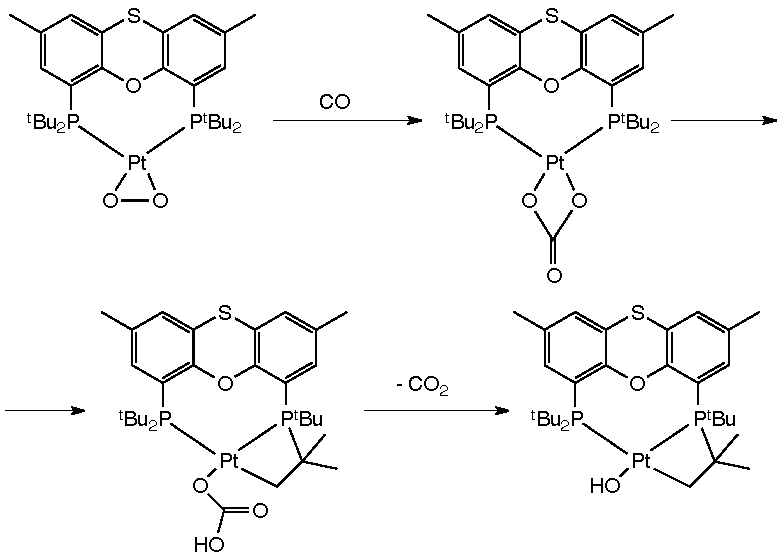
\includegraphics{../Schemes/StBuPtO2andCO.pdf}
\caption[Reaction between \ce{[Pt(tBu-thixantphos)O2{]}} and CO]{Reaction between \ce{[Pt(tBu-thixantphos)O2{]}} and CO.}
\label{scheme:StBuPtO2andCO}
\end{center}
\end{scheme}

Unlike previously reported carbonate complexes \ce{[Pt(tBu-thixantphos)CO3]} reacts further. 
A down-field peak is observed in the proton NMR at 17.6 ppm indicating the presence of an acidic proton.  There are also two phosphorus peaks at 50.5 ppm and -38.7 ppm with satellites of 1893 and 2854 respectively.  The upfield shift of one phosphorus is commonly associated with metallation of a tertiary butyl group.\cite{Garrou1981}  Based on this data intemediate \fixme{reference} is proposed. 

Intermediate \fixme{give a reference} then loses carbon dioxide (enriched when using \carbon{}O) to give the final product \fixme{reference}.  The final product is asymmetric and retains the metallacycle from the \fixme{reference} previous compound.  The two phosphines appear at 38.2 (\JPtP{} = 1794 Hz) and -49.6 ppm (\JPtP{} = 3943 Hz).  The small coupling constant for the non-metallated carbon indicates that it is trans to a ligand with a strong trans influence, in this case the metalled t-butyl group.  The metalled phosphorus shows the significant downfield shift expected for metallation.  The identity of the final ligand has not been conclusively identified.  The large coupling constant for the metallated carbon suggests a ligand with a weak trans influence such as a halide or an oxygen donor.  The mass spec gives a signal for [M-L]\textsuperscript{+} so is of little assistance.  A hydroxyl ligand is the likely by-product from the loss of \ce{CO2} from fix me{reference}, and we would expect that a hydroxyl may well exchange with deuterium and be broad in the \proton{} NMR thus explaining the absence of the signal.  

The final two structures are particularly note-worthy due to the cis-coordination of the phosphines.  Such sterically bulky ligands show a distinct preference for trans-coordination (as we will see in \fixme{reference to platinum(II) stuff}).  The metallacyclobutane must be cis, however the ligand could still maintain a trans coordination.  It is likely that the coordination plane is distorted and the phosphines are not perfectly 90 \degrees{} thus allowing for pseudo-cis coordination.  In addition the metallation of the t-butyl may hold that part of the molecule in a particular geometry resulting in less steric hindrance for the other phosphine.  

\fixme{check if metallacycles can include phosphines or just carbons and metals}

\section{Reactions with Palladium(0) Precursors}

Attempts to synthesise palladium(0) complexes were much less successful than the work with platinum(0).  Reaction between \ce{Pd2dba3} and tBu-thixantphos resulted in a single complex which showed similarities to the platinum xantphos dioxygen complexes that formed from the 14-electron complex.  A single product at 40.0 ppm in the \phosphorus{} NMR spectrum was observed and did not appear to have any associated dba.  However, the was unable to be separated from the uncoordinated dibenzylideneactone by-product. \fixme{my Pt(O2) complex is insoluble in benzene and dba probably is soluble so maybe washing with some toluene might be enough? Or crystallisation from toluene}

Cyclopentadiene palladium allyl is often used as a palladium(0) precursor in catalytic reactions as the reductive elimination of the cyclopentadiene and the allyl generates a palladium(0) and an inert \fixme{C8H8?} alkyl which is generally unreactive towards the catalyst.  Reaction between cyclopentadiene palladium allyl and tBu-thixantphos was attempted with little success.  A number of products were observed with peaks appearing at 33.5, 42.9 and 51.9 ppm in the \phosphorus{} NMR spectrum in addition to the dioxygen complex which forms over times at 40.0 ppm.  The major product is the broad signal at 42.9 ppm which may be an allyl complex or something?

The \carbon{} NMR spectrum showed signals at 147.2 and 145.1 ppm which have previously been seen with this ligand for the proton adjacent to the phosphine selenide.  This significant shift is a result of close proximity to a heavy atom so it may be that a very unusual coordination has formed including perhaps dimers or oligomers?  It is also possible that there may be an allyl or something strange forming \fixme{check for free cp} perhaps some sort of propene structure?

An alternative route to palladium(0) could include the reaction with trisnorbornene palladium which would be an exact analogue of the successful reaction with trisnorbornene platinum.  Another attempt could be via the reduction of the relatively easy to synthesise dichloropalladium tBu-xantphos complexes.  However reduction of palladium dichlorides requires a cis-coordination of the chlorides if this is not the case then the chlorides are often substituted for hydride ligands.\fixme{try this and see what happens with [Pd(tBu-thixantphos)Cl]}.  In this case however, due to the lability of palladium and one of the chloride ligands it may be that it can reorganise to a pseudo-cis configuration for the reduction or I may form a dihydride.  It is also possible that this is atmosphere dependent and that doing the reaction in the air may result in the Pd(0) dioxygen complex.  

\section{Reactions with Platinum(II) Precursors}

The coordination chemistry with platinum(0) was shown to produce a number of platinum(II) complexes upon reaction.  Metal(II) complexes are often used as precatalysts so we decided to investigate the coordination behaviour of the tBu-xantphos ligands with metal(II) precursors.  

\subsection{Reactions with platinum dichloride starting materials}

Metal halide complexes are ubiquitous in coordination chemistry.  They form a number of catalytic complexes and are widely used as starting points for more complex systems.  Platinum halide complexes are also of interest due to their potential for use as chemotherapeutics such as the commonly employed cis-platin, now an important part of a wide range of treatment protocols.\fixme{reference?}  

The reaction with platinum dichloride starting materials formed exclusively the \emph{trans}-dichloride platinum diphosphine complexes regardless of the geometry of the starting material and no evidence for \emph{cis}-chelation was observed at any point throughout the reaction.  \fixme{reference}  This is highly unusual for diphosphine ligands.  The ability to form \emph{trans}-chelates is rare for diphosphines and those that can typically form a mixture of \emph{cis} and \emph{trans}-geometries.\cite{Freixa2008}  Xantphos itself almost exclusively forms \emph{cis} chelates and the few examples of \emph{trans}-chelation of xantphos that do exist are unstable or form as mixtures with the \emph{cis}-chelates. \fixme{references and structures?}

The trans- platinum tBu-thixantphos dichloride complex that formed shown a solvent dependent NMR spectrum.  In \ce{C6D6} a single sharp peak was observed at 32.9 ppm (\JPtP = 2700 Hz) in the \phosphorus{} NMR spectrum.  However, in \ce{CD2Cl2} or \fixme{acetone?} this peak became very broad.\fixme{check this stuff}  The polar solvent would be likely to stabilise an ionic species more than nonpolar benzene, we theorised that an equilibrium was present between the dichloride and a mono chloride species (Scheme \ref{scheme:chloridedissociation})

\begin{scheme}[ht]
\begin{center}
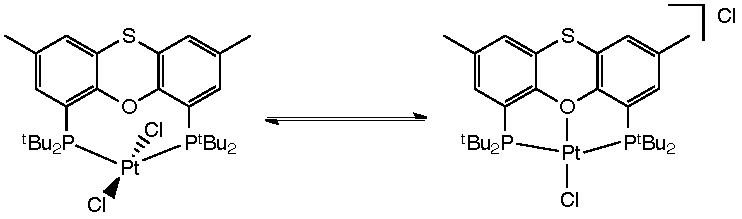
\includegraphics{../Schemes/Chloridedissociation.pdf}
\caption[Equilibrium between \ce{[Pt(tBu-thixantphos)Cl2]} and \ce{Pt(tBu-thixantphos)Cl]Cl}]{Equilibrium between \ce{[Pt(tBu-thixantphos)Cl2]} and \ce{Pt(tBu-thixantphos)Cl]Cl}}
\label{scheme:chloridedissociation}
\end{center}
\end{scheme}

The choice of starting material was shown to be very important to the speed of the reaction.  A large number of different starting materials were investigated with nitrile, thioether, alkene and chloride leaving groups.  An overview of reaction conditions and results are given in Table \ref{table:dichloridestartingmaterials}.  The fastest of the dichloride materials investigated was \ce{[Pt(hex)Cl2]} this starting material is often used as alkene bind weakly to platinum and are readily displaced by phosphines.  Interestingly although this is a \emph{cis}-dichloride and the product is a \emph{trans}-dichloride the \ce{[Pt(hex)Cl2]} reacted much faster than any of the other precursors.  This is likely a result of the ease of substitution of platinum alkenes relative to platinum nitriles or thioethers.  \fixme{try Zeise�s dimer?}

\begin{table}[ht]
\caption[Reaction of tBu-thixantphos with various platinum dichloride precursors]{Reaction of tBu-thixantphos with various platinum dichloride precursors}
\label{table:dichloridestartingmaterials}
\begin{center}
\begin{tabular}{l l l l l}
	\toprule
	~~Starting Material~~ 	&~~Solvent~~	&~~Temperature~~	&~~Time~~	&~~Yield (by NMR)~~\\
	\midrule		
~~Pt(hex)Cl2			&		&		&		&	\\
~~Pt(hex)I2			&		&		&		&	\\
~~PtCl2(SEt2)2			&		&		&		&	\\
~~PtCl2(MeCN)2 -cis?	&		&		&		&	\\
~~PtCl2(MeCN)2 - trans	&		&		&		&	\\
~~PtCl2(tBuCN)2 - trans	&		&		&		&	\\
~~K2[PtCl4]			&		&		&		&	\\
	\bottomrule{}
\end{tabular}
\end{center}
\end{table}

Although a vast number of platinum dichloride starting materials were investigated the reactions were generally carried out in CDCl3 so they mostly just formed the protonated ligand.  However it looks like PtCl2(tBuCN) reacted with the protonated ligand that formed - maybe worth trying this again in something like benzene or acetone. 

In order to test the chloride dissociation theory we dissolved the complex in acetone and reacted with ammonium hexafluorophosphate.  The solution changed over 30 minutes from deep orange to yellow and a precipitate of ammonium chloride formed.  The product appeared at 46.4 ppm (\JPtP = 2347 Hz) in the \phosphorus{} NMR spectrum with an associate septet at -144.5 ppm indicative of \ce{PF6}.  The platinum phosphorus coupling constant had dropped from the dichloride complex by 353 Hz.  This indicates that the phosphorus atoms are still in a trans configuration but they are more strongly bound to the platinum \fixme{?}  As the platinum has lost a chloride ligand it will have less electron density and thus will bond more strongly to the phosphines to compensate.  A shift in the \carbon{} NMR spectrum for the carbon adjacent to the ether bridge also occurred from 155.8 ppm to 157.4 ppm.  This downfield  shift is indicative of a deshielding of the carbon centre.  This deshielding may be the result of oxygen coordination as the oxygen donates electron density to the platinum it will pull electron density from the surrounding carbons resulting in deshielding of those carbons.  The \carbon{} NMR resonance for the aromatic carbon \emph{ipso} to phosphorus has shifted significantly upfield from 124.5 to 119.1 ppm.\fixme{why?}

The relationship between these two compounds was further studied by variable temperature \phosphorus NMR analysis \fixme{figure?}.  A sample of \ce{[Pt(tBu-thixantphos)Cl2]} in \ce{CD2Cl2} was analysed down to -80 \degC.  At room temperature a single broad resonance at 32.9 ppm was observed.  Upon cooling down to -20 \degC this resolved into a single sharp peak, however cooling further led to the conversion of this dichloride into the monochloride appearing at 46.4 ppm.  The mono chloride became the major product below approx -60 \degC.  This may be due to the steric influence of the chlorides and the diphosphine.  At room temperature and above the complex has sufficient energy to exchange between the dichloride and monochloride complexes resulting in a single broad peak.  However upon lowering the temperature the dichloride is preferred.  Lowering further preferences the monochloride.  This effect is likely sterics, at the lower temperature the complex has less energy to move and thus prefers a structure with sufficient space to for all of the ligands around the platinum.  

\subsubsection{Reactions of Pt(POP)Cl}

Hybrid ligands have attracted attention recently due to their combination of different bonding atoms which can lead to differing activity in the trans positions.  If one of the ligating atoms is a weak donor group then the ligand can also exhibit hemilability where the weakly bonding ligand can be displaced by something else (such as a reagent in a catalytic reaction) but the ligand still remains anchored to the metal centre and can thus still influence the reaction and can recoordinate rapidly once the reaction is complete thus stabilising the resting state for the catalyst.  

The complex \ce{[Pt(POP)Cl]PF6} where POP = tBu-thixantphos bonding through the two phosphines and the oxygen.  Has the potential for hemilability of the ether bridge.  This was investigated by reaction with carbon monoxide (Scheme \fixme{draw a scheme}).  The first complex is as expected where the carbon monoxide displaces the oxygen and coordinates to the platinum centre.  However, this then reacts (most likely with adventitious water) to displace the chloride and form a hydride complex.  This complex is only stable under an excess of carbon monoxide and readily loses CO and the oxygen recoordinates thus demonstrating hemilability.  Using \carbon{} enriched carbon monoxide allowed for further characterisation.  Selected NMR data for these compounds are summarised in Table \fixme{put a table here}.

\subsection{Reactions with platinum dimethyl starting materials}

Metal alkyl complexes form as intermediates in a wide range of catalytic transformations including polymerisation reactions and C-H activation.  If methane underwent C-H activation on a platinum centre then a platinum methyl complex would be formed.  These complexes are also interesting for their potential protonation to form a sigma-methane complexes similar to that reported by Brookhart.\cite{Bernskoetter2009}  

tBu-Thixantphos was reacted with \ce{[Pt(hex)Me2]} in a benzene solution.  Even with high temperatures \fixme{check what they were} and extended reaction times no reaction was observed.  An equivalent of acid was added to attempt to promote loss of methane and coordination of the diphosphine, however the acid reacted exclusively with the diphosphine instead of \ce{[Pt(hex)Me2]}.  In order to form a complex, Initial reaction between the diphosphine and \ce{[Pt(hex)Me2]} may form a complex with a dimethyl and a monodentate phosphine and hexadiene (Scheme \ref{scheme:dimethyl}).  If this forms then the steric bulk resulting from two bidentate ligands in monodentate coordination may destabilise the complex thus favouring loss of the monodentate phosphine to reform the starting materials rather than rearrangement of the strongly bound methyls into a trans configuration.

\begin{scheme}[ht]
\begin{center}
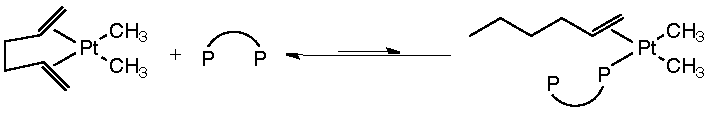
\includegraphics{../Schemes/Dimethyl.pdf}
\caption[Proposed reaction between \ce{[Pt(hex)Me2]} and a diphosphine ligand]{Proposed reaction between \ce{[Pt(hex)Me2]} and a tBu-xantphos diphosphine ligand (abbreviated PP)}
\label{scheme:dimethyl}
\end{center}
\end{scheme}

\subsection{Reactions with Platinum Chloro Methyl starting materials}

Reaction with \ce{[Pt(hex)ClMe]} is much faster than either the \ce{[Pt(hex)Cl2]} or \ce{[Pt(hex)Me2]}.  This may be due to the faster reorganisation to a \emph{trans} geometry as a result of the stronger \emph{trans} influence of the methyl to promote loss of the chloride.  A single product is observed as a single sharp peak in \ce{d6-acetone} at 50.5 ppm (\JPtP{} = 2793 Hz).  This indicates \emph{trans}-coordination of the diphosphine.  Contrary to the reaction with \ce{[Pt(hex)Cl2]}, the complex that forms exclusively is a tridentate methyl complex (Scheme \ref{scheme:platinumchloromethyl}).  Due to the high \emph{trans} influence of the methyl the loss of the chloride is promoted and this is the only product even without the addition of \ce{NH4PF6} to promote the reaction.  

\begin{scheme}[ht]
\begin{center}
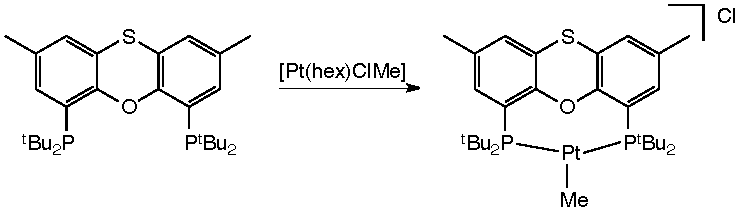
\includegraphics{../Schemes/Platinumchloromethyl.pdf}
\caption[Reaction between \ce{[Pt(hex)ClMe]} and tBu-thixantphos]{Reaction between \ce{[Pt(hex)ClMe]} and tBu-thixantphos}
\label{scheme:platinumchloromethyl}
\end{center}
\end{scheme}

The platinum methyl appears in the \proton{} NMR spectrum at 1.56 ppm as a triplet (coupling to both phosphorus atoms) with platinum satellites of 97.4 Hz.  This is very large for a two-bond platinum coupling and is indicative of a very weakly bound group \emph{trans} to the methyl.  Similar complexes reported previously include \fixme{reference ingleson2004 and others?} which have similar platinum couplings.  However the resonance for the methyl in the \carbon{} NMR spectrum is present at -23.8 ppm as a triplet with platinum satellites of 777.2 Hz.  To the best of our knowledge this is the largest reported platinum coupling constant to a methyl carbon.  All of this data supports the structure proposed as not having an interaction between the oxygen and the platinum.  Although there may be one present it is very weakly bound.  The most similar NMR data has platinum methyls \emph{trans} to weakly bound agostic interactions of isopropyl or t-butyl groups.  In these cases no evidence of the agostic interaction was seen in the NMR spectra it was only observed in the X-ray crystal structure.  Low temperature NMR down to -80~\degC{} showed no evidence for an agostic interaction.  It is also likely that as t-Bu thixantphos has an oxygen present close to the platinum that this would coordinate preferentially to forming an agostic.  

\fixme{make sure that all of this is good}  

\section{Reaction with palladium(II) precursors}







